\subsection{Subsistema de alimentación}

El subsistema de alimentación es el encargado de permitir que el sistema se alimente a través de baterías. También permite cargar la batería e incluso ambas acciones simultáneamente.

Como batería hemos decidido utilizar una batería de ion de litio 18650, un modelo bastante estándar en las aplicaciones integradas.  Concretamente, hemos decidido utilizar el modelo \texttt{INR18650-29E} de Samsung, que tiene una tensión nominal de 3.7\ V y una capacidad de 2900\ mAh.

Sin embargo, este tipo de baterías tienen unos requisitos de carga muy estrictos. Contando con que la batería parte de un estado correcto (no por debajo del límite de tensión segura), se debe cargar primero con un método de corriente constante hasta alcanzar una tensión cercana a la máxima y después cambiar a un método de tensión constante hasta finalizar la carga \cite{BU409ChargingLithiumion}. Un ejemplo de ciclo de carga se puede ver en la \autoref{fig:2-1-cicloCarga}

\begin{figure}[h]
    \centering
    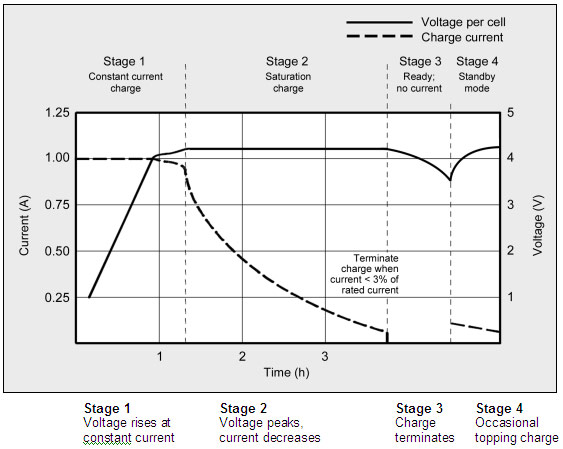
\includegraphics[width=0.5\textwidth]{images/2/2-1/cargaBateria.png}
    \caption{Ciclo de carga de una batería de ión de litio}
    \label{fig:2-1-cicloCarga}
\end{figure}

Si no se respeta el ciclo de carga de estas baterías, se tiene una alta probabilidad de que falle de forma violenta, siendo incluso un peligro de incendio. 

\subsubsection{Circuito de carga}

Para facilitarnos la tarea de respetar este ciclo hemos utilizado una solución integrada de Texas Instruments, el \texttt{BQ25606}, un cargador de una celda de litio que soporta hasta 3 amperios de corriente. \cite{BQ25606DataSheet}

Gracias a este circuito integrado y bastantes componentes externos, podemos diseñar un circuito que, a partir de una tensión de entrada entre 5 y 12 voltios y utilizando un convertidor reductor, carga la batería adecuadamente y de forma segura. 

La entrada al circuito puede ser a través de un conector \textit{Jack} de alimentación o un conector \textit{Micro USB}. Además, si se utiliza el segundo conector, el integrado se encarga de negociar el protocolo de carga rápida con la fuente de alimentación para incrementar la corriente de entrada y mejorar la potencia de carga. 

Además, si el circuito está conectado a la alimentación y la fuente tiene suficiente capacidad, la corriente de salida se obtiene de la entrada en lugar de la batería, gracias a la tecnología PowerPath de TI. Esta tecnología además permite balancear las tres corrientes, por lo que si el sistema requiriera de más corriente de la que la fuente de alimentación pudiera proveer, se obtendría también de la batería realizando un esfuerzo coordinado entre la fuente y la batería. Si por el contrario la fuente puede ofrecer más corriente de la que se está solicitando en la salida, se utiliza este excedente para cargar la batería.

Este circuito cuenta además con dos indicadores LED que informan sobre si la fuente de alimentación está conectada y las tensiones son correctas (verde en nuestro circuito) y si se está cargando la batería o hay algún fallo (roja en nuestro circuito). La segunda luz se mantiene encendida mientras se está cargando, se apaga cuando se ha finalizado la carga y parpadea a 1 Hz de frecuencia si hay algún error.

Para ofrecer todas estas características, el circuito integrado consta de una máquina de estados finitos y múltiples comparadores de error. Con esta inteligencia conmuta tres transistores para conectar la batería y para gestionar el convertidor conmutado síncrono que se construye. Se puede ver un diagrama de bloques resumido del circuito (obtenido de la hoja de catálogo) en la \autoref{fig:2-1-bloquesInternosBQ25606}

\begin{figure}[h]
    \centering
    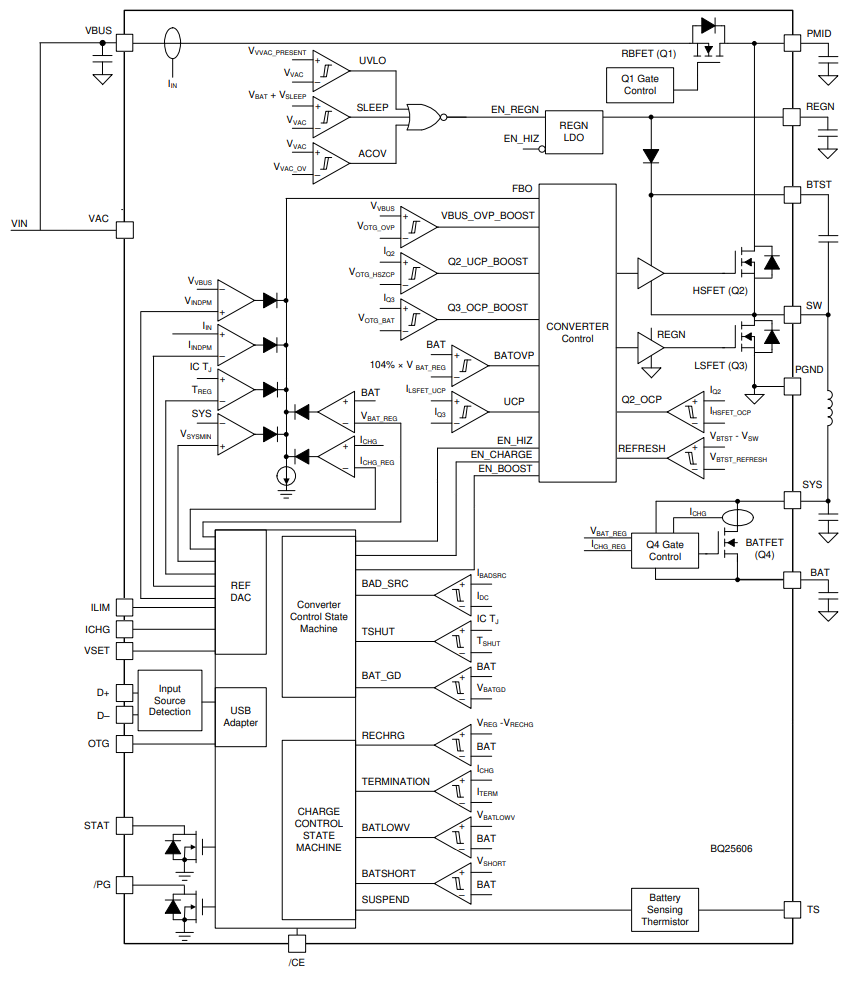
\includegraphics[width=0.5\textwidth]{images/2/2-1/BQ25606Bloques.png}
    \caption{Diagrama de bloques interno del BQ25606}
    \label{fig:2-1-bloquesInternosBQ25606}
\end{figure}

Este circuito ofrece a su salida una tensión aproximadamente igual a la de la batería durante el funcionamiento normal, por lo que está alrededor de los 3.7 V. Sin embargo, si la tensión de la batería cae por debajo de 3.5 V, el circuito se encarga de ofrecer dicha tensión a la salida, por lo que nunca bajará de dicho valor (mientras la batería puede ofrecer corriente y no esté descargada).

El circuito integrado ofrece también la posibilidad de utilizar una batería con sensor de temperatura integrado, pero no vamos a utilizarlo debido al incremento en coste de la misma.

En la hoja de catálogo del integrado se ofrece información sobre el proceso de diseño de un circuito alrededor de dicho integrado. Además, se tiene una nota de aplicación sobre el diseño de circuitos alrededor de este integrado \cite{texasinstrumentsDesigningStandaloneSingle}:

\begin{itemize}
    \item Inductancia de 2.2 $\mu$ F para reducir el rizado de corriente.
    \item Pin \texttt{VSET} flotante para tensión de carga máxima de 4.208 V.
    \item Divisor de tensión de dos resistencias de 10 $k\Omega$ en \texttt{TS} para no utilizar divisor de tensión.
    \item Resistencia de 165 $\Omega$ en \texttt{ILIM} para limitar la corriente de entrada cuando no se negocia carga rápida a 3 A (normalmente se utiliza mucho menos).
    \item Resistencia de 487 $\Omega$ en \texttt{ICHG} para limitar la corriente de carga máxima a 1.4 A como se indica en las especificaciones de la batería.
    \item El resto de componentes se toman de la Figura 10-1 de la hoja de catálogo
\end{itemize}

Por tanto, esta parte del circuito queda como se puede ver en la \autoref{fig:2-1-circuito-carga-final}.

\begin{figure}[h]
    \centering
    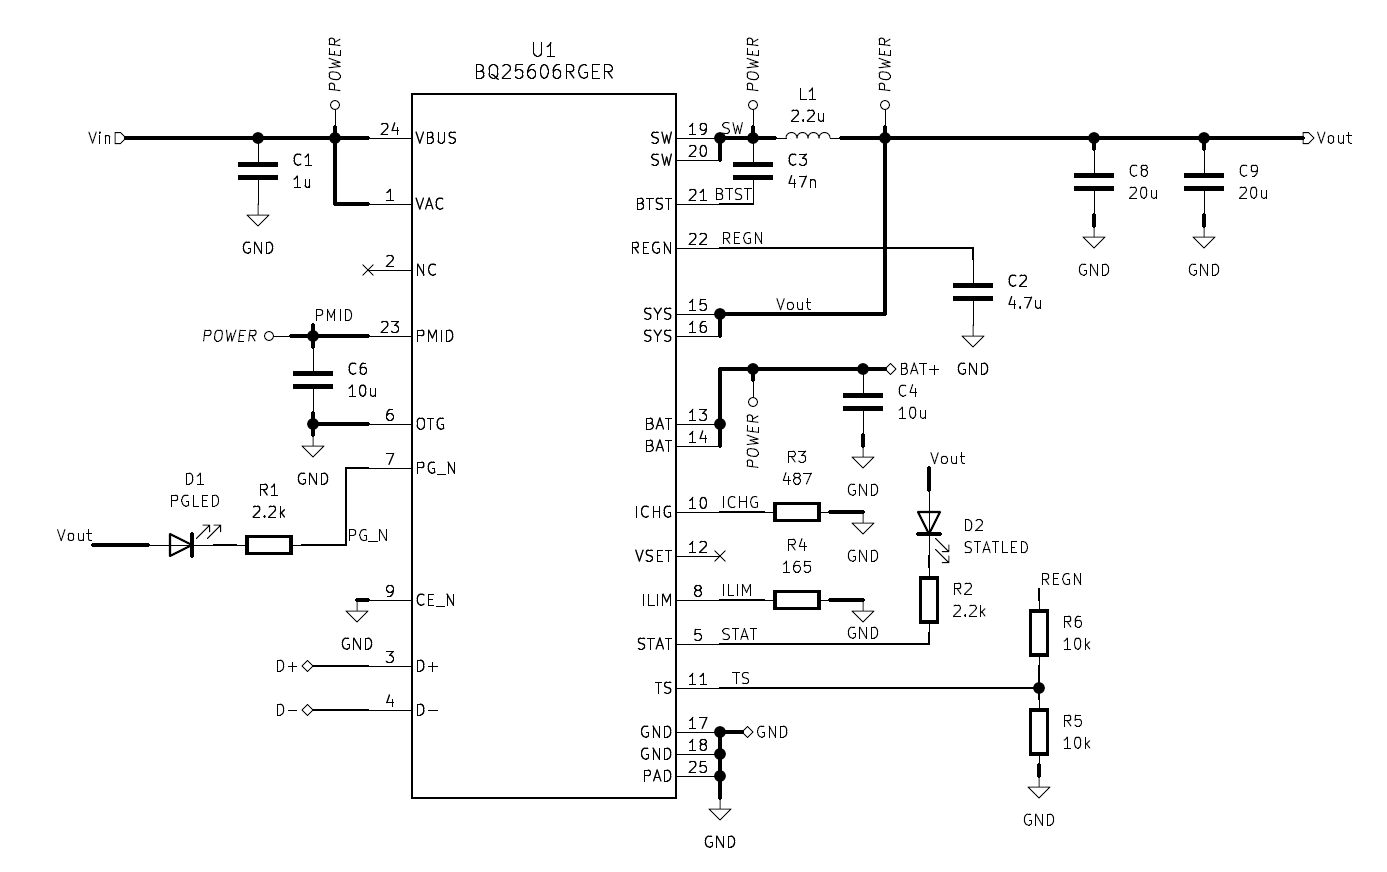
\includegraphics[width=\textwidth]{images/2/2-1/circuitoCarga.png}
    \caption{Subcircuito de carga de batería}
    \label{fig:2-1-circuito-carga-final}
\end{figure}

\subsubsection{Convertidor elevador}\label{subsubsec:convertidor_elevador}

La placa que utilizamos especifica una tensión de entrada de 7 V a 12 V si se utiliza el pin $V_{in}$ inferior. Preferimos utilizar este método ya que la entrada de 5 V no tiene protección y se puede dañar la placa si no se realiza todo el proceso adecuadamente.

Experimentalmente hemos notado que la placa utiliza la misma corriente de entrada para cualquier valor de tensión, por lo que seguramente utilice un convertidor de tensión lineal internamente para generar las tensiones. Por tanto, hemos preferido tomar el valor más pequeño de las tensiones de entrada para reducir la pérdida de potencia.

La tensión de salida del circuito de carga oscila entre los 3.5 V y los 4.2 V, por lo que hemos diseñado un convertidor conmutado elevador o \textit{Boost Converter} para obtener dicha tensión a partir de la salida del cargador.

Un circuito convertidor elevador está compuesto básicamente por una bobina, un transistor y un controlador PWM.\ Como controlador PWM hemos utilizado otra solución integrada de Texas Instruments debido a la alta precisión que nos permite tener, ya que un fallo en este circuito podría dañar seriamente al resto del sistema. 

El circuito integrado elegido es el LM51561H. Este circuito es un controlador de convertidores conmutados de tipo \textit{Boost, SEPIC} y \textit{Flyback} con gran rango de tensiones y muy elevada protección. \cite{LM51561HDataSheete}

Además, indica específicamente que está pensado para aplicaciones de batería gracias a su baja tensión de entrada necesaria para funcionar. Al contrario que el circuito del cargador, este integrado no incluye los transistores internos por lo que se tienen que añadir externamente. 

Este integrado consta básicamente de comparadores de error respecto a tensiones de referencia y un generador de señales triangulares para la generación de PWM. Cuenta además con la posibilidad de compensar el circuito para evitar su inestabilidad. La versión LM51561H es igual que la LM5156H solo que con protección en modo \textit{Hiccup}. En este modo de protección, si se detecta una sobrecarga, se desactiva el convertidor y se comienza una espera. Al finalizar la espera, se trata de volver a arrancar la conversión. Si la condición de sobrecarga sigue presente, se vuelve a dormir y repetir el ciclo. Esto permite una mucho menor potencia media en condición de sobrecarga en comparación a la protección por corriente media, pico o valle. \cite{hariImprovePowerConverter}

Se puede ver un diagrama de bloques resumido en la \autoref{fig:2-1-LM51561H-bloques}.


\begin{figure}[h]
    \centering
    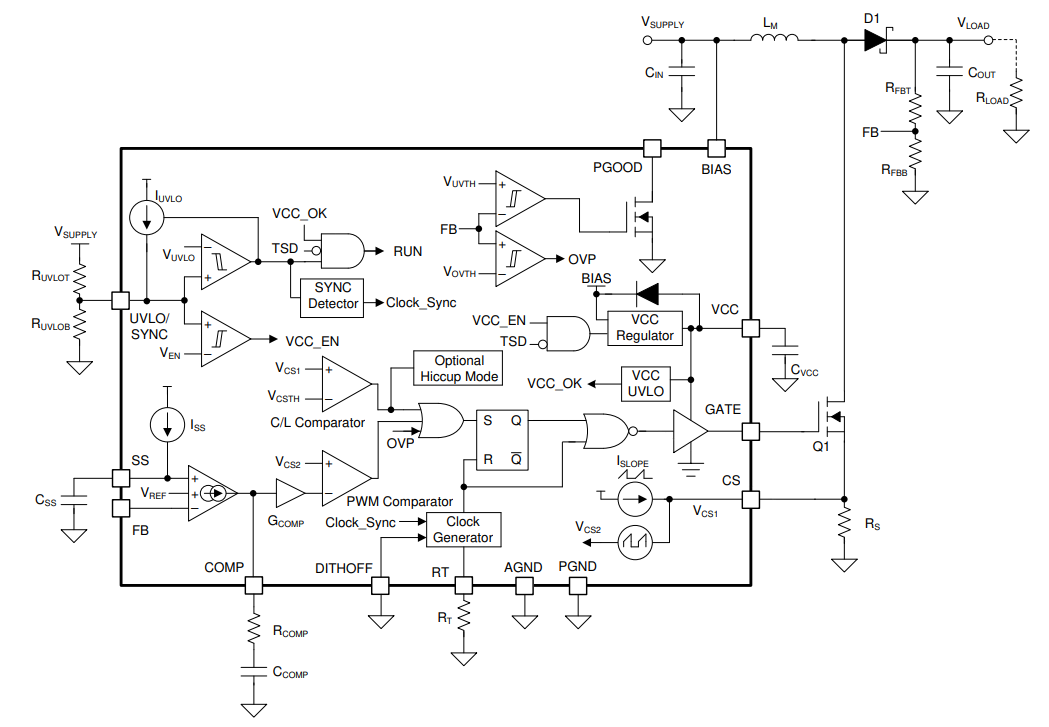
\includegraphics[width=0.5\textwidth]{images/2/2-1/LM51561HBloques.png}
    \caption{Diagrama de bloques interno del LM51561H}
    \label{fig:2-1-LM51561H-bloques}
\end{figure}

Algunas de las características destacables de nuestro circuito son:
\begin{enumerate}
    \item Protección contra infravoltaje (\textit{Undervoltage Lockout}). Se comprueba que el pin \texttt{UVLO} tenga una tensión superior a 0.55 V para comenzar la configuración interna y superior a 1.5 V para comenzar a conmutar.
    \item Frecuencia elevada de conmutación para evitar interferencias en las bandas de AM y reducir las pérdidas de conmutación.
    \item Salida de 7 V muy estable y con poca dependencia de la corriente de salida
\end{enumerate}

Para el diseño de este circuito, el fabricante recomienda el uso de la herramienta WEBENCH Power Designer\footnote{\url{https://www.ti.com/tool/download/SNVC224}}, que permite reducir la complejidad del diseño realizando los cálculos necesarios para los parámetros deseados y la compensación de la función de transferencia del circuito. 

Utilizando dicha herramienta, generamos el circuito que hemos utilizado con los siguientes parámetros: 
\begin{enumerate}
    \item $V_{in, \min} = 3.5\ V$
    \item $V_{in, \max} = 4.2\ V$
    \item $V_{out} = 7.0\ V$
    \item $I_{out} = 1.0\ A$
\end{enumerate}

Una vez introducidos los parámetros, el software genera el circuito con los componentes recomendados, permitiendo sustituirlos por equivalentes y generando las gráficas de funcionamiento aproximado. Se puede encontrar el reporte generado en el \autoref{anexo:webench-report}

Con el resultado de dicho software, se construye un circuito como el de la \autoref{fig:2-1-circuito-boost-final}.

\begin{figure}[h]
    \centering
    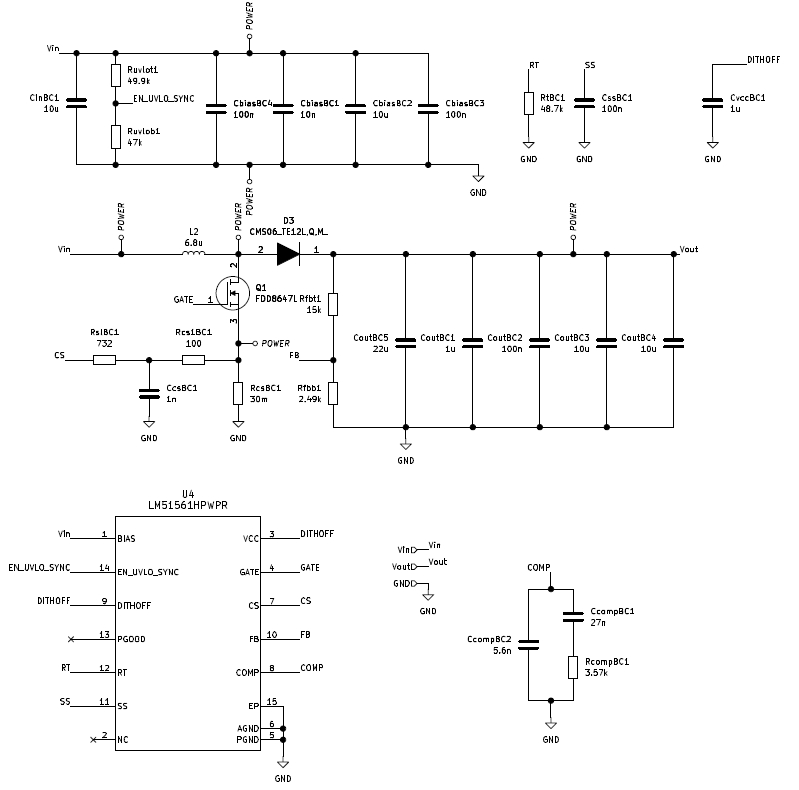
\includegraphics[width=0.5\textwidth]{images/2/2-1/circuitoElevador.png}
    \caption{Circuito del convertidor elevador}
    \label{fig:2-1-circuito-boost-final}
\end{figure}

\subsubsection{Medidor de consumo}
\label{subsubsec:medidor-consumo-analog}

Otra parte importante de este circuito es el medidor de consumo integrado. Para ello, primero pensamos en construir un amplificador de instrumentación, que se puede adquirir ya implementado en un mismo paquete o realizar con dos amplificadores operacionales. Sin embargo, durante la búsqueda de modelo de amplificador operacional encontramos un modelo que se ofrece como especializado en medición de corriente en el nivel bajo (\textit{Low-side current switching}) por lo que decidimos quedarnos con él.

Dicho integrado es el OPA187ID, un amplificador operacional de precisión con aproximadamente cero tensión de offset ($10\ \mu V$, $0.001\mu V/^\circ\! C$). \cite{OPA187DataSheet}

Dicho amplificador operacional recomienda montar una configuración de amplificador diferencial con una resistencia \textit{shunt} de muy baja impedancia y configurar la ganancia deseada mediante las resistencias de realimentación.

Como resistencia de medida hemos elegido un valor bajo, de $10\ m\Omega$ y que soporta 1 W de potencia. Para simplificar los cálculos, hemos decidido asignar el rango de entrada de un ADC de nuestra placa ($[0, 3.3]\ V$) a un rango de $[0, 3]\ A$. Por ello, la ganancia es:

\[
    G = \frac{3.3 - 0}{3 - 0} = 1.1 V/A  
\]

Para conseguir dicha ganancia es tan sencillo como utilizar resistencias con un cociente de 110, por lo que elegimos valores de $1\ k\Omega$ y $110\ k\Omega$ en el circuito, por lo que obtenemos el circuito de la \autoref{fig:2-1-medidor-consumo}.

\begin{figure}[h]
    \centering
    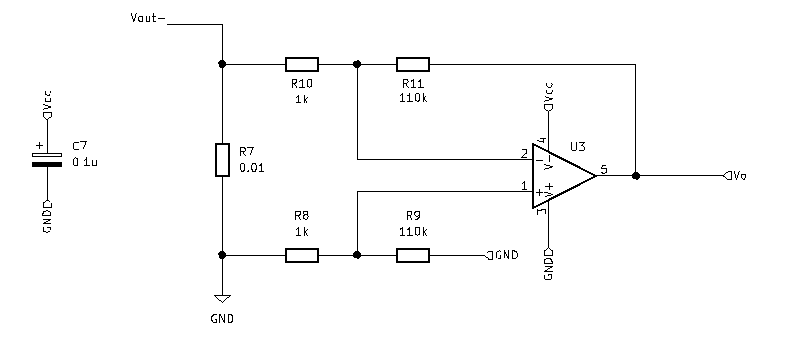
\includegraphics[width=0.5\textwidth]{images/2/2-1/circuitoConsumo.png}
    \caption{Circuito medidor de consumo}
    \label{fig:2-1-medidor-consumo}
\end{figure}

\subsubsection{Diseño de PCB}

Los tres circuitos se han integrado en una sola PCB, permitiendo una mucho mejor integración y uso mucho más sencillo. Se ha integrado un zócalo para insertar la batería sobre la placa y evitar la posibilidad de una mala conexión. Además, se han incluido los conectores de entrada de potencia previamente mencionados, tanto el Jack de alimentación como el conector micro-USB. Por otro lado, la salida del sistema se realiza a través de unos terminales de tornillo que incluyen la tensión de alimentación positiva, negativa y la medida de consumo.

Sin embargo, por un problema durante el ensamble de la placa, se destruyeron los pads del conector micro-USB, por lo el conector no funciona correctamente. Sin embargo, el sistema funciona perfectamente a través del Jack de alimentación.

La alta complejidad de los circuitos integrados hace que sus empaquetados sean muy pequeños, por lo que la soldadura se ha tenido que realizar mediante horno y con stencil. Sin embargo, esto nos ha permitido colocar los componentes muy próximos entre sí, reduciendo el ruido electromagnético generado y las componentes parásitas del circuito. Concretamente, el circuito integrado de carga es de empaquetado \texttt{VQFN24} con un tamaño de $4x4\ mm$ y el integrado del conversor es \texttt{HTSSOP14} con un tamaño de $5x4.4\ mm$.

Además, el pequeño tamaño de estos circuitos reduce significativamente su capacidad de disipación térmica. Por ello, ambos incluyen un pad en su parte inferior que debe ser soldado a un pad que además incluya muchas vias térmicas a la capa inferior, en la que debe haber un plano de tierra grande para disipar el calor que se genere. Por ello y para ofrecer un camino de retorno a las altas corrientes que recorren este circuito, la capa inferior se dedica casi exclusivamente a la masa del circuito. 

Ambos circuitos integrados ofrecen indicaciones sobre la disposición de los componentes que se han seguido rigurosamente. Por ejemplo, se recomienda mantener los bucles de conmutación lo más pequeños posibles o mantener separadas las tierras digital y analógica, juntandolas únicamente en un punto. 

Ciertas zonas del circuito han tenido que ser diseñadas mediante polígonos especiales al no poderse realizar la conexión mediante pistas normales o necesitar zonas especialmente grandes para caminos de mucha corriente.

Se puede ver el resultado final del circuito de alimentación en la \autoref{fig:2-1-circuito-alimentacion}.

\begin{figure}[h]
    \centering
    \includegraphics[width=0.5\textwidth]{images/2/2-1/circuitoAlimentación.jpg}
    \caption{Circuito de alimentación}
    \label{fig:2-1-circuito-alimentacion}
\end{figure}

Se tiene un esquema completo del circuito en el \autoref{anexo:circuito-alimentacion}